% !TEX root = ../Thesis.tex

\chapter{Spin Defects}

\section{Electron Spin Resonance}
\subsection{Spin States}

Paramagnetic defects in crystals are one of the major experimental areas under investigation as potential qubit platforms. This thesis will focus on the paramagnetic defects found in two semiconductor crystals: silicon and diamond. In silicon, neutrally charged group V donors offer a system analogous to a Hydrogen atom: a single unpaired electron bound to a nucleus with a net positive charge. Both electron and nucleus in this system have the property of intrinsic angular momentum or \emph{spin}, $\mathbf{S}$, a vector property of the system with components $S_x, S_y, S_z$. The projection of the particle's spin along any given axis is one of a series of discrete values dependent on the total spin of the system and spaced by integer values of $\hbar$. Typically and from here $\hbar$ is treated as being equal to 1 for ease of calculations. The electron is a spin-$\frac{1}{2}$ particle and can take only the values (or eignestates) $-\frac{1}{2},\frac{1}{2}$. A nucleus, however, may have a variety of different spin values. Phosphorus donors in silicon have a spin-$\frac{1}{2}$ nucleus whilst Bismuth donors have a spin-$\frac{9}{2}$ nucleus. As the $S_{x,y,z}$ operators are non-commuting, the spin can have a defined value in only one cartesian dimension, usually defined as $S_z$. For a free electron, not in the presence of a magnetic field, space is isotropic, meaning any axis can be specified as $S_z$ and the two eigenstates $\pm\frac{1}{2}$ are degenerate in energy.

Associated with the spin of a particle is a magnetic dipole moment, $\mathbf{\mu}$, that determines the degree of interaction between the particle and a magnetic field, known as the Zeeman interaction \cite{10003989896}. For an electron, this moment, $\mu_e$, is equal to $-g\mu_b\mathbf{S}$ where $\mu_b$ = $\frac{e\hbar}{2m_e}$. The energy of this dipole interacting with a magnetic field, $\mathbf{B}$, is then equal to $-g\mu_b\mathbf{S}\cdot\mathbf{B}$. In practice the $S_z$-axis of the spin is defined as being aligned with the magnetic field giving two spin eigenstates. The Hamiltonian governing the electron spin can then be written:

\begin{equation}
H = -g\mu_bB_0S_z
\label{eq:freeelecham}
\end{equation}

Where $B_0$ is the magnitude of the magnetic field $|\mathbf{B}|$. This Hamiltonian then gives two spin eigenstates, designated as $\ket{0}$ and $\ket{1}$ or $\ket{\uparrow}$ and $\ket{\downarrow}$, corresponding to the spin being aligned and anti-aligned with the magnetic field. The energy difference between these states is:

\begin{equation}
\Delta E = g_e\mu_bB,
\label{eq:enSplit}
\end{equation}

This results in an energy splitting as seen in figure \ref{fig:elecSplit} a. Typically, the energy level splittings are referred to by their frequency, according to the equation $E = h\nu$, as this gives the frequency of a microwave pulse resonant with the transition.

In practice, electrons bound to defects in semiconductors are not free, and cannot be described fully by the simple Hamiltonian shown in \ref{eq:freeelecham}. The chief reason for this is that the electron will be bound to a nucleus with its own spin state, $\mathbf{I}$. To account for the nucleus, the Hamiltonian requires the addition of two further terms: one to account for the hyperfine interaction and one to account for the nuclear spin's interaction with the magnetic field. The hyperfine interaction refers to the effect of the magnetic fields from electron and nucleus interacting with each other. This interaction leads to two possible energy states, where electron and nuclear spin are aligned (higher energy) and where they are anti-aligned (lower energy). Due to the small nuclear magneton, $\mu_N$ of the nucleus, the hyperfine interaction is typically a significantly greater energy effect than that of the nuclear Zeeman term, except at very high magnetic fields (>1~T). The full Hamiltonian of the electron-nuclear spin system can be written as follows \cite{landlifquantmech}:

\begin{equation}
  \hat{H} = -g\mu_b\mathbf{B}\cdot\mathbf{S} + g_I\mu_N\mathbf{B}\cdot\mathbf{I} + \hat{A}\mathbf{S}\cdot\mathbf{I}
  \label{eqn:phos-ham}
\end{equation}

The energy level structure of a phosphorus donor in silicon is described by this Hamiltonian. The phosphorus nucleus, like the electron, is a spin-$\frac{1}{2}$ system ($I = 1/2$), meaning that the joint system has a four level  structure shown in figure \ref{fig:elecSplit}b. At low magnetic fields, this has a singlet ($m_s = 0$) - triplet ($m_s = 1$) structure, due to the dominance of the hyperfine splitting term over the Zeeman terms. At these low fields the spin projection in the $B_0$ direction ($S_z$) of the electron and nucleus does not represent a good quantum number - meaning that the projection will \emph{not} remain constant under time evolution, instead it is their total spin that best represents the system state. At high magnetic fields, where the Zeeman term dominates, the degeneracy of the triplet state is lifted and four well defined energy levels emerge. At these high fields the spin states of electron and nucleus are isolated, meaning their $z$-projection is a good quantum number. Most experiments with phosphorus donors in silicon are performed at these high fields.

\begin{figure}
\centering
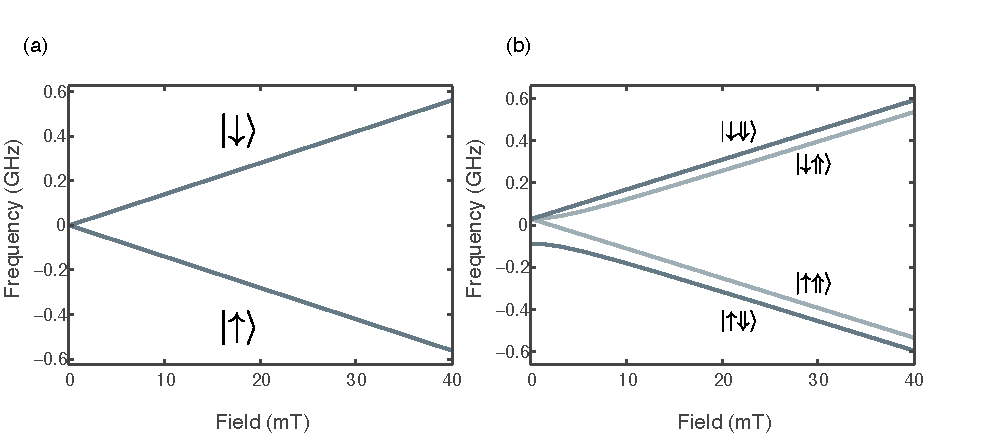
\includegraphics[width = \columnwidth]{Plotting/Figs/all-levels-fig.pdf}
\caption[Energy level splittings for a free electron and an electron bound to a phosphorus donor in silicon]{(a) the energy level splitting of a free electron in a magnetic field, showing how separation in energy increases with magnetic field. (b) the energy level splitting of the spin states of a phosphorus spin system in a magnetic field. $\ket{\uparrow}$ refers to the electron spin state and $\ket{\Uparrow}$ to the nuclear spin state. Note the lower energy state of the anti-aligned nuclear spin state for a given electron spin state, due to the dominance of the hyperfine coupling term over the nuclear Zeeman term in equation~\ref{eqn:phos-ham}.}
\label{fig:elecSplit}
\end{figure}

In addition to causing this level splitting, the magnetic field will also cause the electron spin to precess about the magnetic field at the Larmor frequency, given by:
\begin{equation}
  \omega_0 = \frac{g \mu_B}{\hbar}B_0
\end{equation}

\subsection{The Bloch Sphere}
\label{seq:blochSphere}

The eigenstates of the electron spin in a magnetic field allow the spin to be described as a two level system and represented on the \emph{Bloch Sphere} \cite{Bloch1946,Schweiger}. The Bloch sphere provides a convenient method for representing and visualising quantum states. The two spin states form a basis and are represented by the kets $\ket{0}$ and $\ket{1}$ corresponding to up and down spin or low and high energy levels. These form the North and South poles of the Bloch sphere resepectively. As well as these two spin eigenstates, any linear superposition of them is also a valid state of the system~\cite{Nielsen:2011:QCQ:1972505}:

\begin{equation}
  \ket{\psi} = \alpha\ket{0} + \beta\ket{1}
\end{equation}

If the condition that $\sqrt{|\alpha^2| + |\beta^2|}$ is met than this state is said to be `pure'. All of these pure states of the system are represented by points on the surface of the Bloch sphere. Mixed states, where some classical uncertainty is taken into account in the states representation, fall inside the sphere.

\begin{figure}
  \centering
  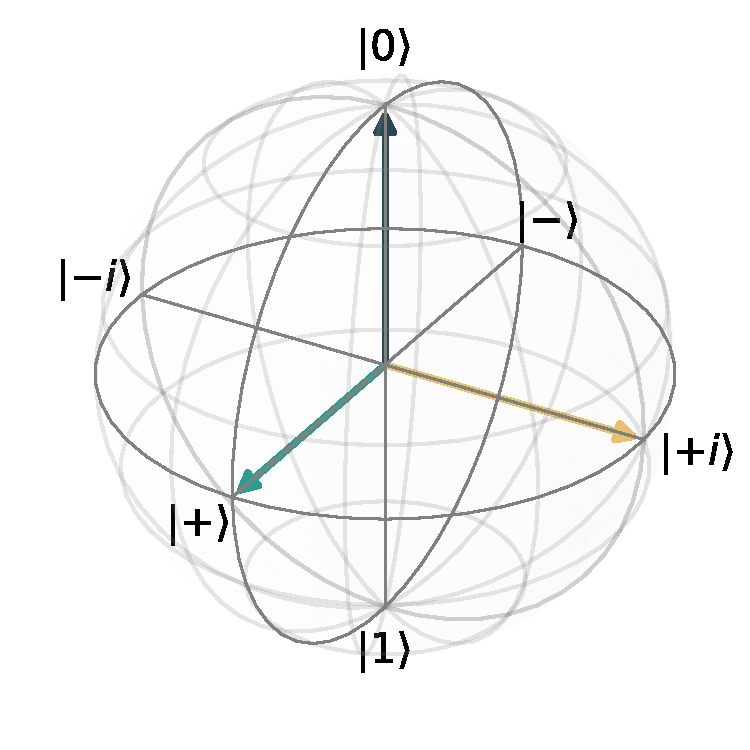
\includegraphics[width=0.5\columnwidth]{/Plotting/Figs/bloch_simple.pdf}
  \caption[The Bloch sphere and Pauli operator eigenstates]{Figure showing the Bloch sphere representation of qubit states. The states shown are the eigenstates of the 3 Pauli spin operators ($S_z \rightarrow [\ket{0}, \ket{1}], S_x \rightarrow [\ket{+}, \ket{-}], S_y \rightarrow [\ket{+i}, \ket{-i}])$, with the states associated with the positive eigenvalue marked by arrows.}
  \label{fig:bloch_simple}
\end{figure}

\subsection{Driving Spin Transitions}


A sufficiently strong static magnetic field, $B_0$, splits the electron energy states and gives the spin eigenstates $\ket{0}$ and $\ket{1}$ but gives no way of driving transitions to other states on the Bloch sphere. To achieve this, a second magnetic field, $B_1$, is typically applied perpendicular to the static field.  The spin will precess around this second magnetic field at the Larmor frequency determined by its field strength~\cite{Schweiger}. A static $B_1$ field can be used as long as the Larmor frequency of this field is significantly faster than that of the $B_0$ field, meaning that precession around $B_0$ can be disregarded whilst the $B_1$ field is applied. In reality, it is not practical to apply such a strong field, so instead a field is applied via an oscillating magnetic field. This will mean that the $B_1$ field will rotate in the $x-y$ plane of the Bloch sphere at $\omega$, the Hamiltonian of this process can then be written:

\begin{equation}
  H = g \mu_B B_0 S_z + g\mu_BB_1 \cos(\omega t)S_x
\end{equation}

For convenience of calculation and understanding, it is typical to perform a transformation on this Hamiltonian into the \emph{rotating frame} by applying the following transformation:
\begin{equation}
  U =
  \begin{pmatrix}
    e^{i \omega t} & 0 \\
    0 & e^{- i \omega t}
  \end{pmatrix}
\end{equation}

This results in the Hamiltonian in the rotating frame being:
\begin{equation}
  \tilde{H} =
  \begin{pmatrix}
    \frac{1}{2}(\omega - \omega_0) & \omega_1 \cos(\omega t) e^{-i \omega t} \\
    \omega_1 \cos(\omega t) e^{i \omega t} & \frac{1}{2}(\omega - \omega_0)
  \end{pmatrix}
\end{equation}

Where $\omega_0$ is the Larmor precession frequency of the $B_0$ field, $\omega_1$ is the precession frequency of the $B_1$ field and $\omega$ is the frequency of oscillation of the $B_1$ field. The counter-rotating terms in the off-diagonal elements of the Hamiltonian can be ignored, as they oscillate quickly relative the the spin (effectively, far off resonance) and so provide only a minor perturbation to its evolution. As such, the final Hamiltonian in the rotating frame can be written:

\begin{equation}
  \tilde{H} =
  \begin{pmatrix}
    \frac{1}{2}(\omega - \omega_0) & \frac{\omega_1}{2} \\
    \frac{\omega_1}{2} & \frac{1}{2}(\omega - \omega_0)
  \end{pmatrix}
\end{equation}

The diagonal elements of this Hamiltonian depend on the detuning between the Larmor precession frequency of the applied $B_0$ field and the frequency of the $B_1$ field and go to 0 when these are on resonance. So the Hamiltonian at resonance is effectively:

\begin{equation}
  \tilde{H} = \frac{\omega_1}{2} \sigma_x
\end{equation}


This allows the precession of the qubit in the static magnetic field to be disregarded, along with the precession of the oscillating $B_1$ field. The application of an on-resonance $B_1$ field will cause a $\ket{0}$ state to precess about the $x$-axis at the Larmor frequency of that field. Off-resonance dynamics are more complex, causing precession about an axis in the Bloch sphere determined by the detuning of the $B_1$ field. As detuning increases, the angle of rotation varies quickly relative to the spin vector, meaning that at large detunings the rotational effect averages out and can be ignored - except in cases where the $B_1$ field is comparable to $B_0$ in magnitude. In most experiments the $|B_1| \ll |B_0|$ requirement holds and the effect of a strongly detuned $B_1$ field can be disregarded. Figure \ref{fig:rabi-dynamics} shows the behaviour of the spin state on the Bloch sphere in the case of both on and off-resonance excitation. The frequency at which the spin rotates in the $B_1$ field when on-resonance is usually termed the \emph{rabi}-frequency and is often designated by $\Omega$. By varying the time the $B_1$ field is applied for, the spin can be rotated to any point on the $z-y$ plane of the Bloch sphere. To perform arbitrary rotations on the Bloch sphere, the phase of the applied $B_1$ field can be varied. This will cause the spin to precess about an axis in the $x-y$ plane, whose angle from the $x$-axis is determined by the phase of the $B_1$ field. By varying this phase and the time the field is applied for it can be used to rotate the qubit to any point on the Bloch sphere.



\begin{figure}
  \centering
  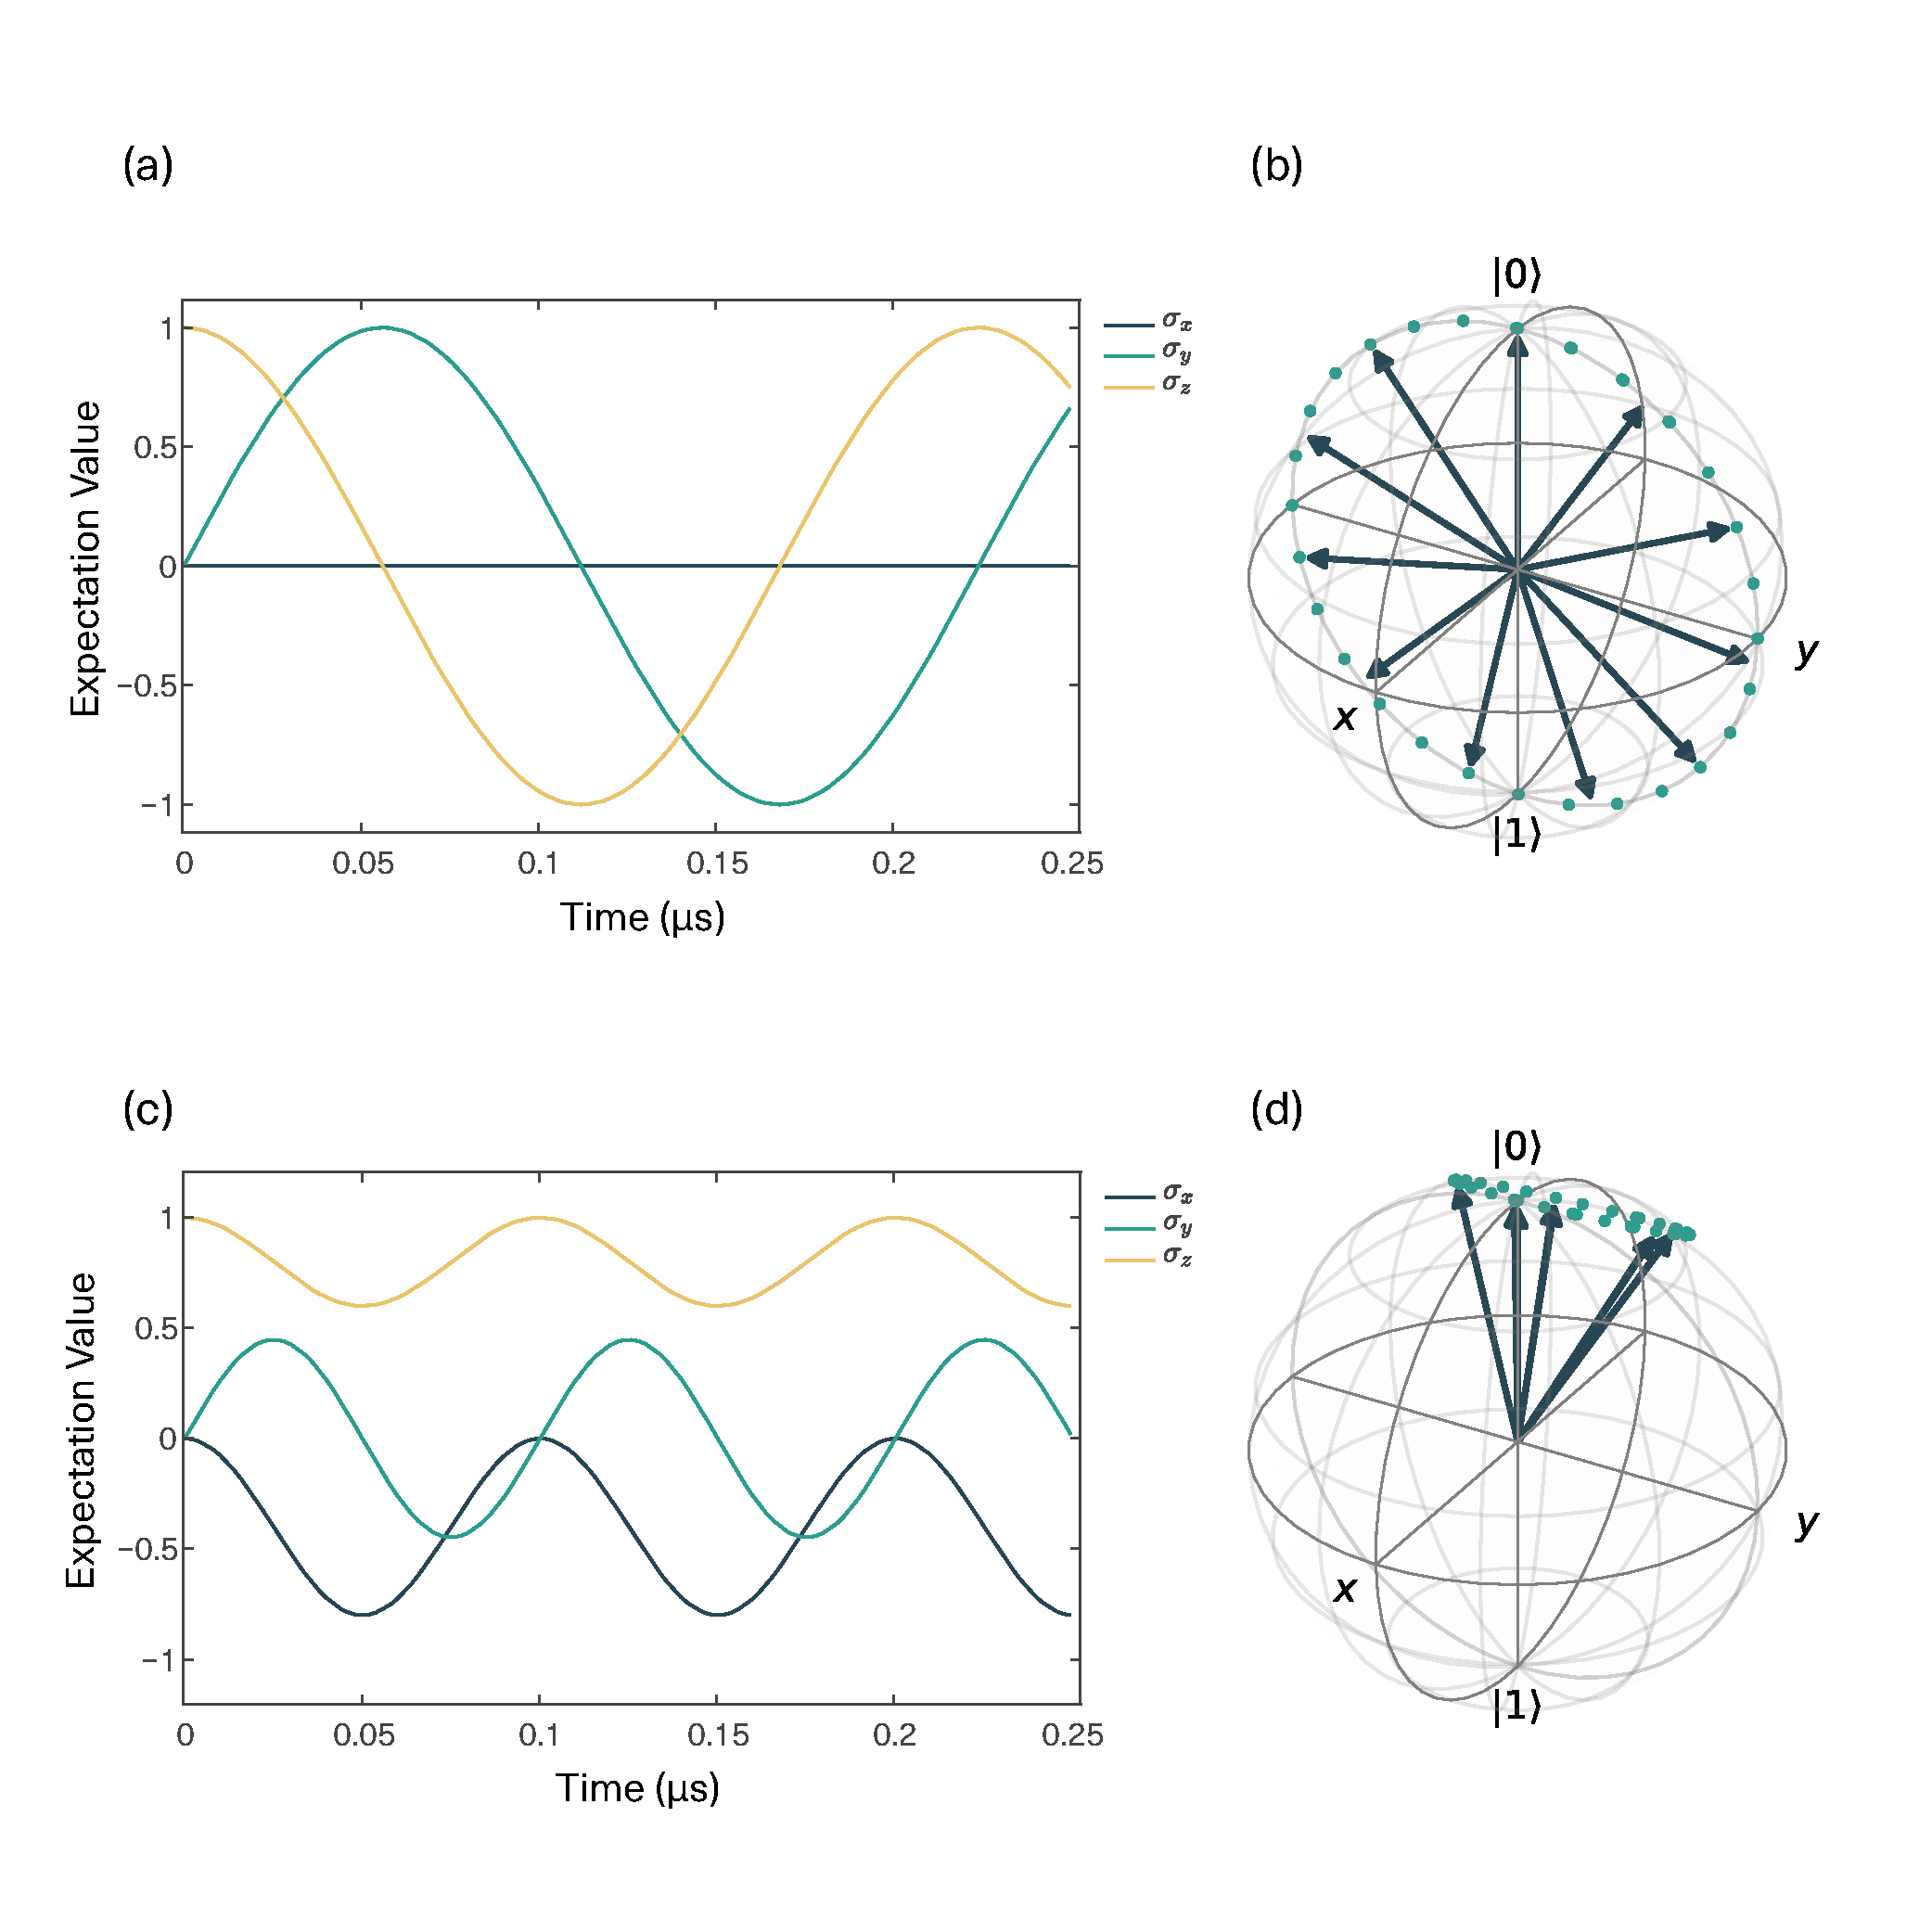
\includegraphics[width=\columnwidth]{/Plotting/Figs/rotating-frame.pdf}
  \caption[Qubit evolution under a an oscillating magnetic field in the rotating frame]{Figure showing qubit evolution under application of an oscillating magnetic field $B_1$, transformed into the rotating frame. In the on resonance case, where the frequency of the $B_1$ field is equal to the Larmor precession frequency of the $B_0$ field, (a) and (b) show the evolution of the expectation values of the Pauli matrices ($\sigma_x, \sigma_y$ and $\sigma_z$) and the state dynamics on the Bloch sphere respectively. (c) and (d) show the same figures for the case of off-resonance excitation, where the $B_1$ frequency is $0.5\%$ lower than the Larmor precession frequency.}
  \label{fig:rabi-dynamics}
\end{figure}

\subsection{Pulsed Electron Spin Resonance}
The processes described above show how a spin can be controlled via the application of magnetic fields, one, $B_0$, splits the electron spin states in energy whilst a second $B_1$ can be used to control the electron spin state. In practice, the process of controlling and measuring the spin states of electron is known as \emph{Electron Spin Resonance} (\textbf{ESR}) or equivalently \emph{Electron Paramagnetic Resonance} (\textbf{EPR}). There are two broad categories of ESR, continuous wave ESR (CW-ESR) and pulsed ESR. Typically, ESR is performed on large ensembles of electron spins, meaning that the behaviour of these spins is somewhat classical in nature as their individual magnetic moments $\mathbf{\mu}$ sum to produce an overall magnetic field vector $\mathbf{M}$.

CW-ESR refers to the process of detecting spin-transitions through the application of a constant oscillating magnetic field to a sample of interest. This field is applied via a resonator and the reflection of this field from the resonator is measured. An external magnetic field is varied and the reflection monitored. Whilst holding the static $B_0$ field constant and varying the $B_1$ field frequency is equivalent in theory, the resonators used for the oscillating fields have narrow ranges of operation meaning that varying the $B_0$ field is much more practical. As the static magnetic field is varied, electron spin transitions may come on resonance with the applied oscillating field, causing less of it to be reflected. This can be detected and the spin transition characterised by its g-factor~\cite{Gere1959,Feher1959}. This form of ESR is not used extensively in this work.

Pulsed ESR does not apply constant $B_1$ fields but instead uses pulses to control spin orientation. As described above, pulse duration (or power) and phase can be varied to rotate the spin vector $M$ to any point on the Bloch sphere. These pulses are usually referred to by their phase the angle of rotation they produce in the spin. So a pulse of duration $\Omega t = \pi$ is termed a $\pi$-pulse and serves to rotate a $\ket{0}$ state to a $\\ket{1}$ state. A $\frac{\pi}{2}$-pulse would rotate a $\ket{0}$ state to a point on the $x-y$ plane of the Bloch sphere.

These pulses provide a means to control the spin states but to be useful for experiments the spin state must be detectable as well. This is done by making use of the precession of the spins in the static magnetic field $B_0$. As these spins precess in the magnetic field they produce a small amount of electromagnetic radiation, with an oscillation frequency equal to their Larmor precession frequency. This radiation can be detected via the resonator that applies the pulses. The amplitude of this radiation is determined by the projection of the precessing spin vector in the $x-y$ plane, so a $\ket{0}$ or $\ket{1}$ produces no signal, whilst a state on the edge of the Bloch sphere in the $x-y$ plane will produce a maximum signal.

In a perfect system, all spins measured in this manner would precess at the same rate and produce a constant signal based on their projection in the $x-y$ plane. However, due to sample imperfections and spacial inhomogeneity in the applied $B_0$ field, each measured spin will precess at slightly different rates. The upshot of this is that the spin signal, made up of multiple signals from many spins, will rapidy lose phase-coherence and the overall signal will go to 0 due to destructive interference between spins rotating with different relative phases. This process is aptly named \emph{dephasing}.

To counteract this, it is possible to use a sequence of pulses to reverse this loss of phase coherence. Whilst many pulse sequences exist the simplest is the spin-echo or Hahn-echo sequence \cite{Schweiger,hahn1950}. This pulse sequence starts with the spin state at $\ket{0}$, where no dephasing occurs, a $\frac{\pi}{2}$ pulse is used to rotate the spin vector to the $x-y$ plane, at which point dephasing begins immediately causing the spin signal to decay. This decaying spin signal is known as \emph{Free Induction Decay} and can be measured to determine the spin state. It is typically not as the sensitive detection equipment used to measure the low-power spin signal can be damaged by high power control pulses, which can remain in the resonator for a short time after the pulse application. Instead the spin ensemble is allowed to dephase in the $x-y$ plane for an amount of time $\tau$ after which a $\pi$ pulse is applied, causing the spin ensemble to invert. The spins now experience the $B_0$ field in reverse and the dephasing they experienced is also reversed. Provided the inhomogeneities that cause the dephasing are constant in time, the spins will rephase after an additional time $\tau$ has ellapsed, causing a brief spike in their signal known as a spin echo. A schematic of this is shown in figure~\ref{fig:hahnechoseq}. A Hahn echo sequence represents the simplest of a broader class of pulse sequences known as \emph{Dynamical Decoupling} or \textbf{DD} sequences, which can be used to protect a spin ensemble or qubit against a variety of different sources of noise.

\begin{figure}
  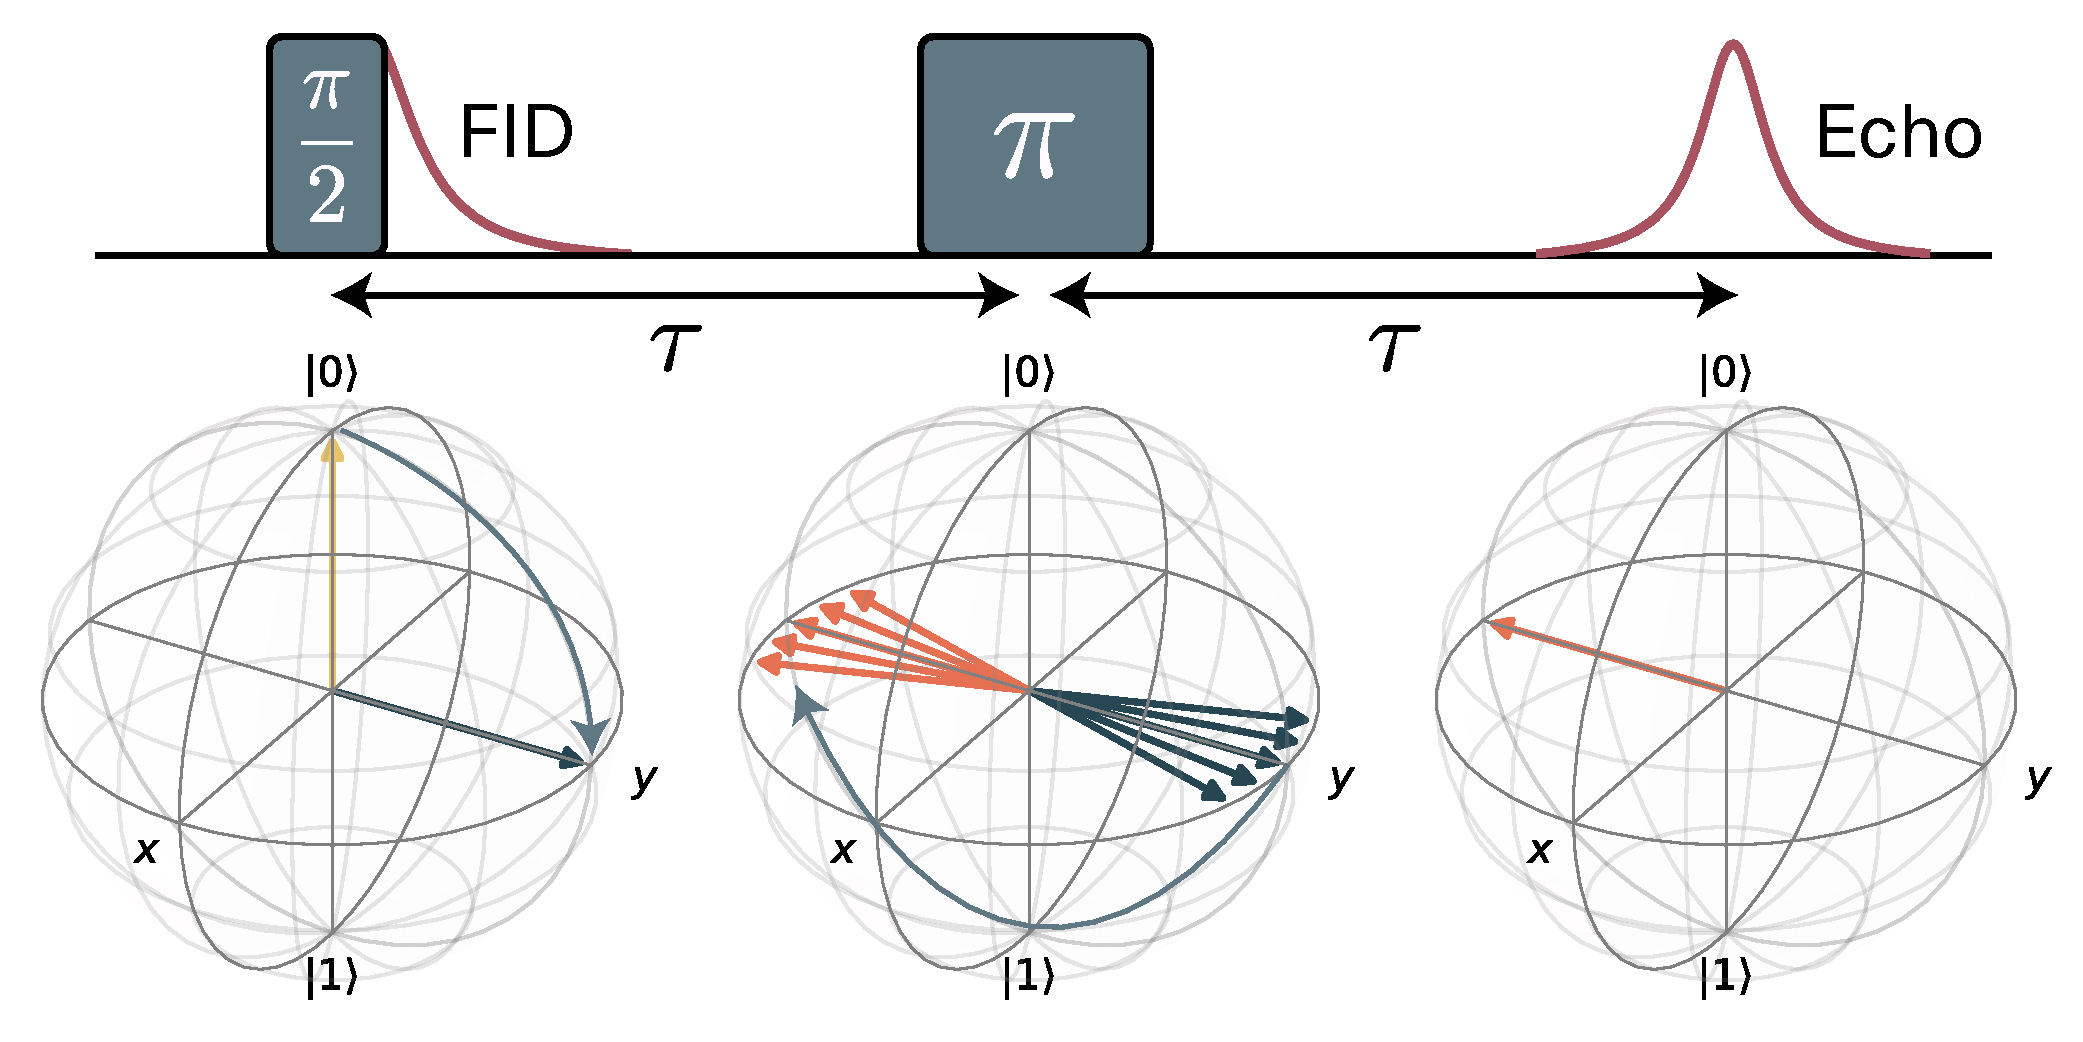
\includegraphics[width=\columnwidth]{/Plotting/Figs/hahn-echo-seq.pdf}
  \caption[Hahn echo sequence and bloch sphere]{Figure showing Hahn Echo sequence and its impact on an ensemble of spins on the Bloch sphere. The pulse sequence is shown above, starting with a $\frac{\pi}{2}$ pulse to take the $\ket{0}$ state into the $x-y$ plane. This then begins to dephase resulting in the rapid loss of signal - observed as the Free Induction Decay or FID. Next a $\pi$ pulse inverts the dephased spins after time $\tau$, causing them to experience a reversed magnetic field and to begin to rephase. After they rephase for another period of $\tau$ their signals interfere constructively once more and the characteristic echo is observed in the signal.}
  \label{fig:hahnechoseq}
\end{figure}

\subsection{Relaxation and Decoherence}

The process of dephasing, described above, introduces the concept of spin ensembles and their loss of phase coherence. This process of dephasing is part of a set of processes by which the ESR signal of an ensemble of spins might be lost or changed over time without control input. Broadly, these processes fall into the categories of \emph{relaxation} or \emph{decoherence} \cite{Schweiger}. Relaxation refers to the processes by which an ensemble of spins disturbed from thermal equilibrium returns to that equilibrium, its timescale is usually referred to as $T_1$. Decoherence refers to the irreversible loss of phase coherence and its timescale is referred to as $T_2$. Dephasing, the reversible loss of phase coherence is characterised by $T_2^*$. Although these processes are understood typically from the point of view of spin ensembles, they have analogous processes when single spins are addressed as well. Relaxation is the process of a qubit returning to its ground state after a certain amount of time. Decoherence is the process of a qubit losing internal phase coherence: the rate at which a superposition state will decay into a maximally mixed state with no quantum nature~\cite{Nielsen:2011:QCQ:1972505}.

\subsubsection{Spin Lattice Relaxation}

The spin relaxation process is most easily understood as the phenomenon that a spin prepared in some state on the Bloch sphere will eventually 'relax' back to the $\ket{0}$ ground state. Spin lattice relaxation is the dominant relaxation process for electron spins in silicon and is caused by the absorption or emission of phonons from the spin into the silicon lattice. From a more intuitive perspective, vibrations in the lattice cause fluctuating magnetic fields that mediate the energy transfer between the spins and the lattice.

As a phonon-mediated process, the dominant determiner of the spin lattice relaxation rate is the temperature of the lattice. There are three main spin-lattice interactions that can cause spin relaxation: \emph{direct, Raman} and \emph{Orbach}~\cite{Schweiger,Orbach1961,Castner1962}.

The direct spin lattice relaxation process is simply the case where the spin absorbs a phonon with frequency equal to the energy of the spin transition. The efficiency of this process is dependent on the phonon and vibrational mode density at the spin transition frequency and temperature, so scales with both. The exact dependence is material specific but at the high magnetic field limit can be approximated by:

\begin{equation}
  T_1 \propto B_0^{-4}T^{-1}
\end{equation}

The direct process is not typically the dominant relaxation process for spins in solids at typical temperatures (>4~K) as maximum phonon density is typically at significantly higher frequencies than the spin transition frequencies. This means that less efficient processes will dominate as more phonons are available to mediate the transition.

The first of these is the two-phonon \emph{Raman} process, whereby the spin first interacts with a phonon of significantly greater energy, $\omega_p$ than the spin transition frequency $\omega_0$. This excites the spin to a virtual excited energy state, before the spin decays back to its ground state by emitting a phonon of energy $\omega_p + \omega_0$. The virtual nature of the energy level allows all phonon energies to mediate this process. The dependence is:

\begin{equation}
  T_1 \propto T^{-9}
\end{equation}

This process is dominant for donors in silicon between 4~K and 10~K.

The final significant process for donor relaxation is the \emph{Orbach} two-phonon process. This is similar to the Raman process but involves the spin being excited to a real energy level rather than a virtual one by a resonant phonon. This process is dependent on the available excited states for the spin, which is donor dependent, and has an exponential dependence:

\begin{equation}
  T_1 \propto e^{-\Delta E / k_b T}
\end{equation}

This Orbach process is dominant in silicon donors at temperatures > 10~K. A schemtic showing the three spin lattice relaxation processes is shown in figure \ref{fig:relaxationprocs}.

\begin{figure}
  \centering
  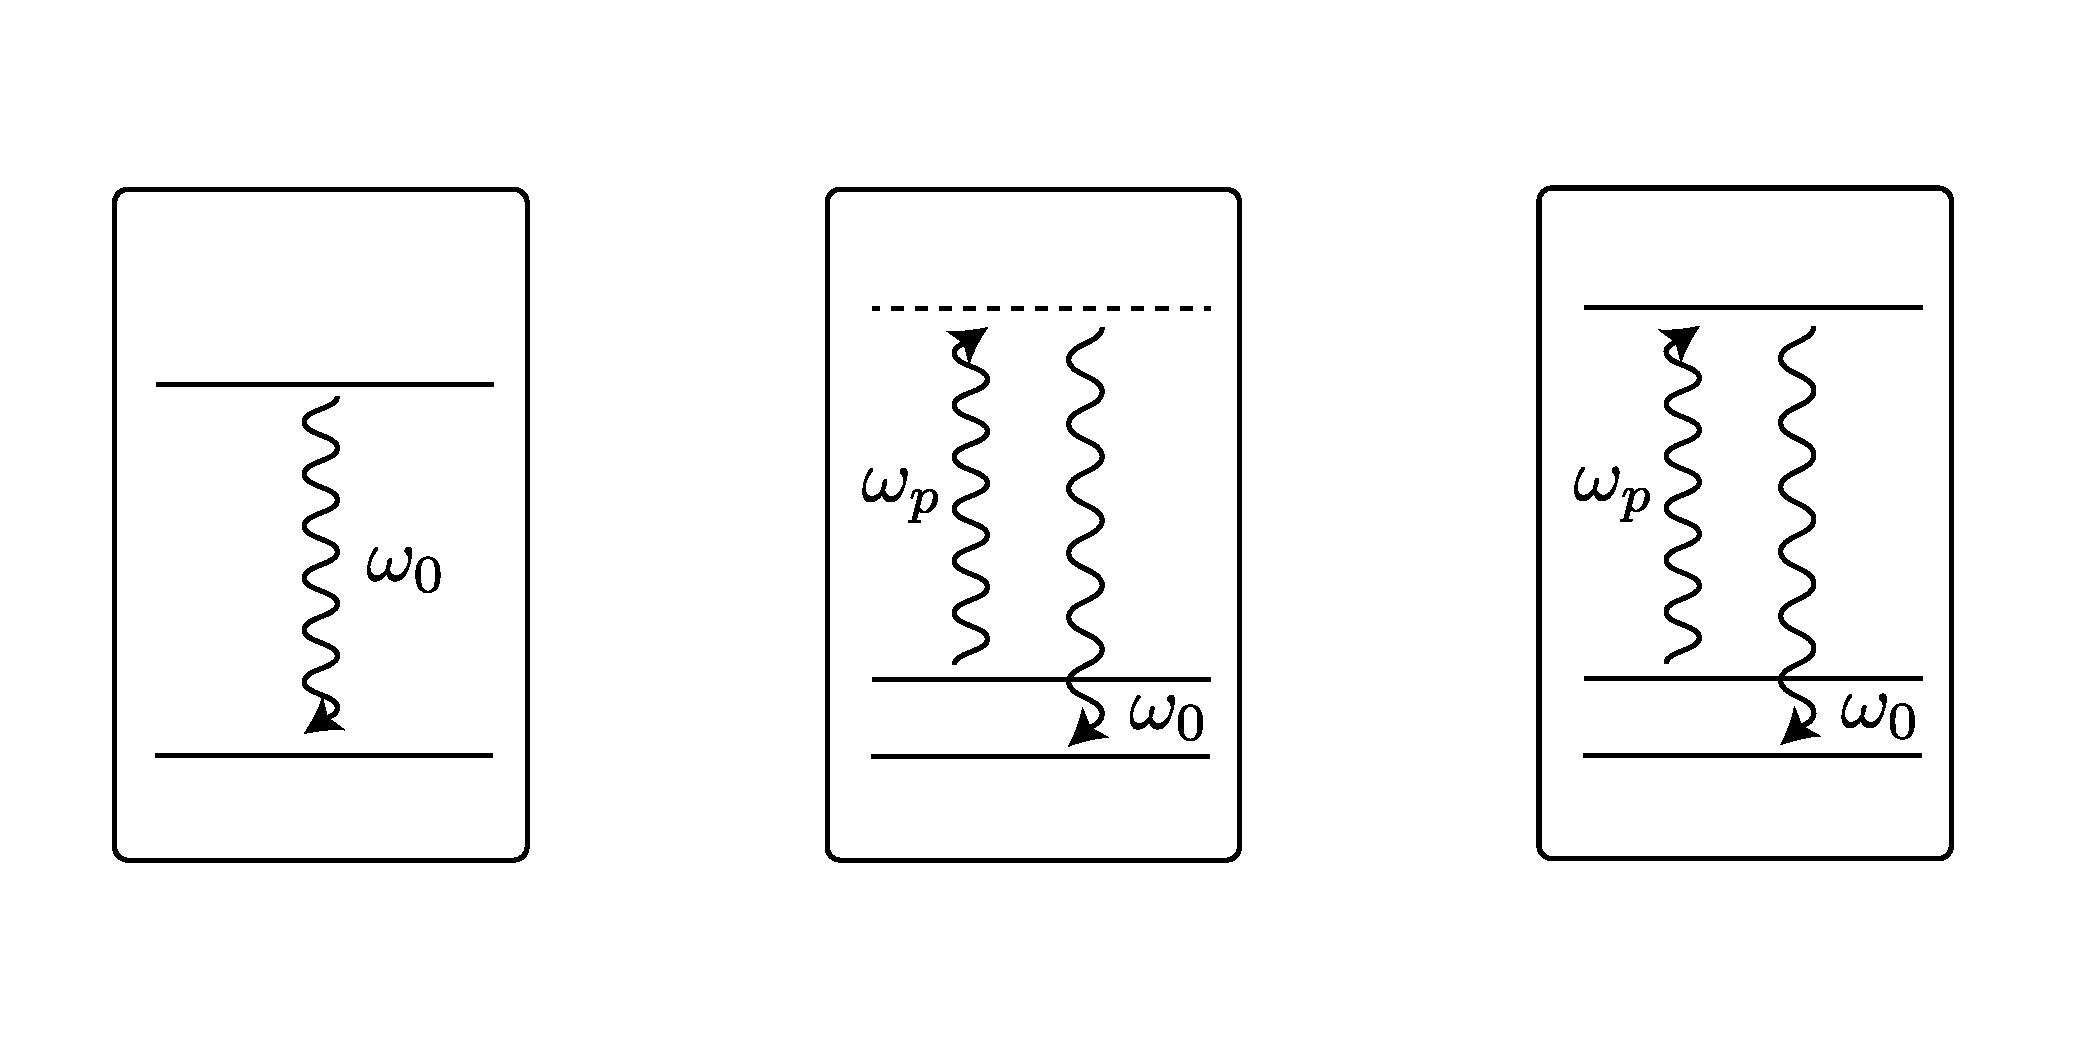
\includegraphics[width=\columnwidth]{/Plotting/Figs/relaxation-processes.pdf}
  \caption[Relaxation processes]{Figure showing simple schematic of the three spin-lattice relaxation processes: \emph{direct, Raman} and \emph{Orbach}. The direct process is dominant below 4~K and involves resonant absorption or emission of a single phonon, the Raman process dominates between 4~K and 10~K and involves non-resonant excitation by a phonon to a virtual energy level before emission of a phonon during relaxation from that energy level. Finally the Orbach process is a resonant two-phonon process requiring excitation to a real energy level before relaxation via phonon emission.}
  \label{fig:relaxationprocs}
\end{figure}

\subsection{Decoherence}


% \subsubsection{Hahn Echo and Detection}
%
% In pulsed ESR the spins are detected via the electromagnetic radiation they emit when precessing in a magnetic field.
% This radiation is of the same frequency as the resonant control radiation (easily shown using equations \ref{eq:enSplit} and \ref{eq:larmor}).
% This emitted radiation can be demodulated with the control radiation giving a DC signal.
% In a perfectly homogeneous magnetic field all spins would precess at the same rate giving a constant DC signal. In reality however, all spins will precess at slightly different rates due to small, static differences in the magnetic field each experiences.
% So, following a $\pi/2$ pulse, the signal from the spins will rapidly decay as the ensemble of spins lose phase coherence.
% A technique, known as a spin or Hahn echo, to reverse this loss of phase was developed by Erwin Hahn in 1950 \cite{hahn1950}.
% This follows a $\pi/2$ pulse with a $\pi$ pulse after a set time interval, $\tau$.
% \textit{Static} magnetic field differences now act to reverse the loss of phase coherence.
% This results in a brief re-phasing of the spins following another interval $\tau$, detected as a rise and fall of a DC signal or an `Echo'.
% A cartoon of this sequence is shown in figure \ref{fig:HahnEcho}.
%
% \begin{figure}
% \centering
% 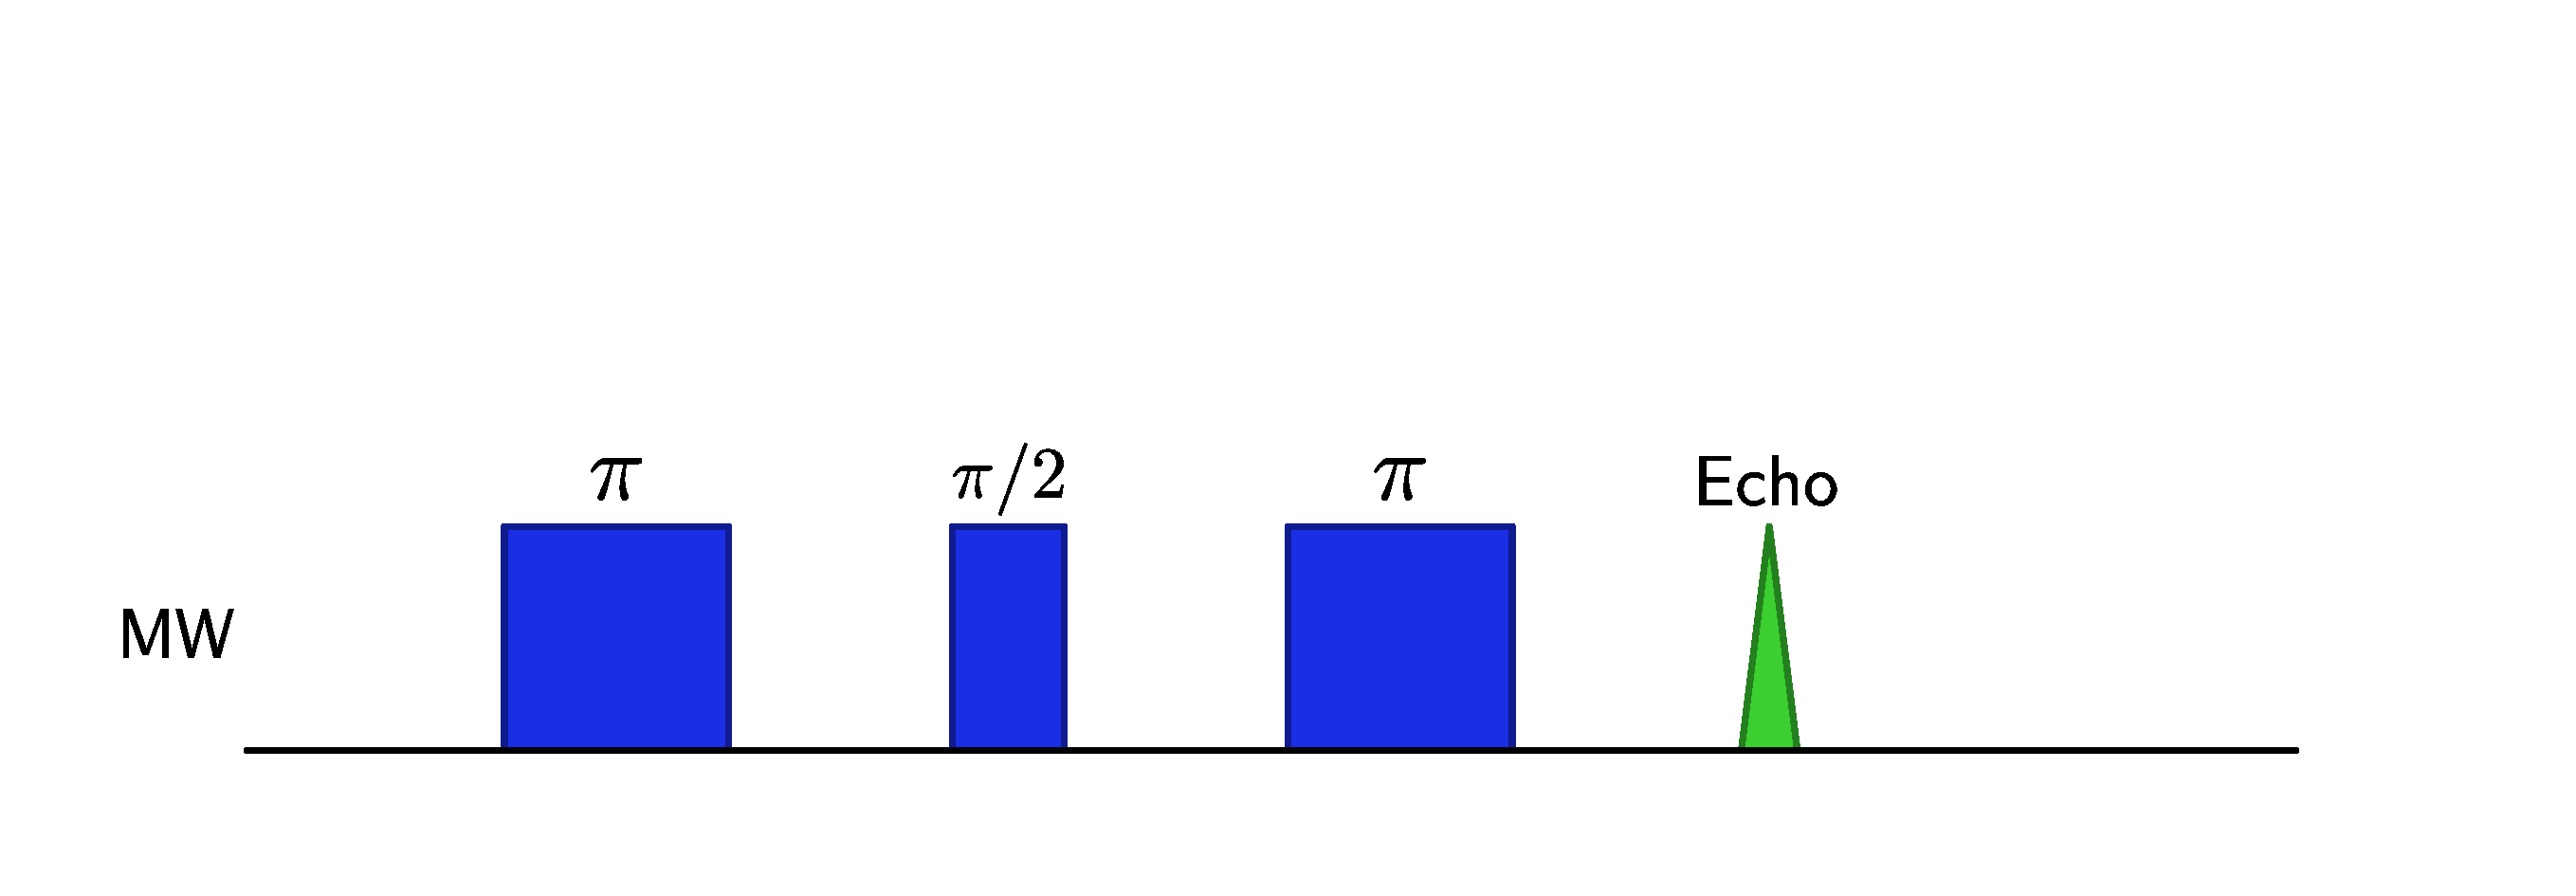
\includegraphics[width = \columnwidth]{Figures/hahnEcho.pdf}
% \caption[Hahn echo sequence]{Cartoon showing a Hahn echo pulse sequence. A $\frac{\pi}{2}$ pulse causes the spins to precess in the $x-y$ plane. Loss of phase coherence is reversed via a $\pi$ pulse following time interval $\tau$ and a signal is detected following another interval of $\tau$.}
% \label{fig:HahnEcho}
% \end{figure}
%
%
% \subsubsection{The Bloch Sphere}
%
% The control pulses produce a magnetic field that rotates at the same rate as the spins, meaning a fixed coordinate system can be defined.
% The rotation axis of the control pulses can be changed by varying their phase, for example a pulse of 0 phase is defined as a rotation about the $x$ axis whilst a pulse of $\pi/2$ phase is a rotation about the $y$.
% This allows control of the direction of the spin vector in 3-D space, with the $z$-axis defined by the static magnetic field.
% A qubit, the basic unit of a quantum computer, can be described as a point within a unit sphere, known as a Bloch sphere and shown in figure \ref{fig:blochSphere} \cite{Nielsen:2011:QCQ:1972505}.
% Clearly then, a single spin is an archetypal qubit: its eigenstates of $\ket{\uparrow}$ and $\ket{\downarrow}$ form the poles of the Bloch sphere.
% Microwave pulses of defined duration and phase enable the creation of an arbitrary linear superposition that allows the initialisation of any state on the surface of the Bloch sphere.
% In the case of ESR, however, a huge number ($10^{10}$) of spins is being addressed.
% Although this means that they do not represent a true qubit, measurements of ensemble properties give great insight into the behaviour of single spins.
% It is therefore prudent to establish the anticipated behaviour of the various potential spin qubit candidates using the comparatively simple experimental techniques of ESR before making the challenging step to single spin control and measurement.
%
% \begin{figure}
% \centering
% 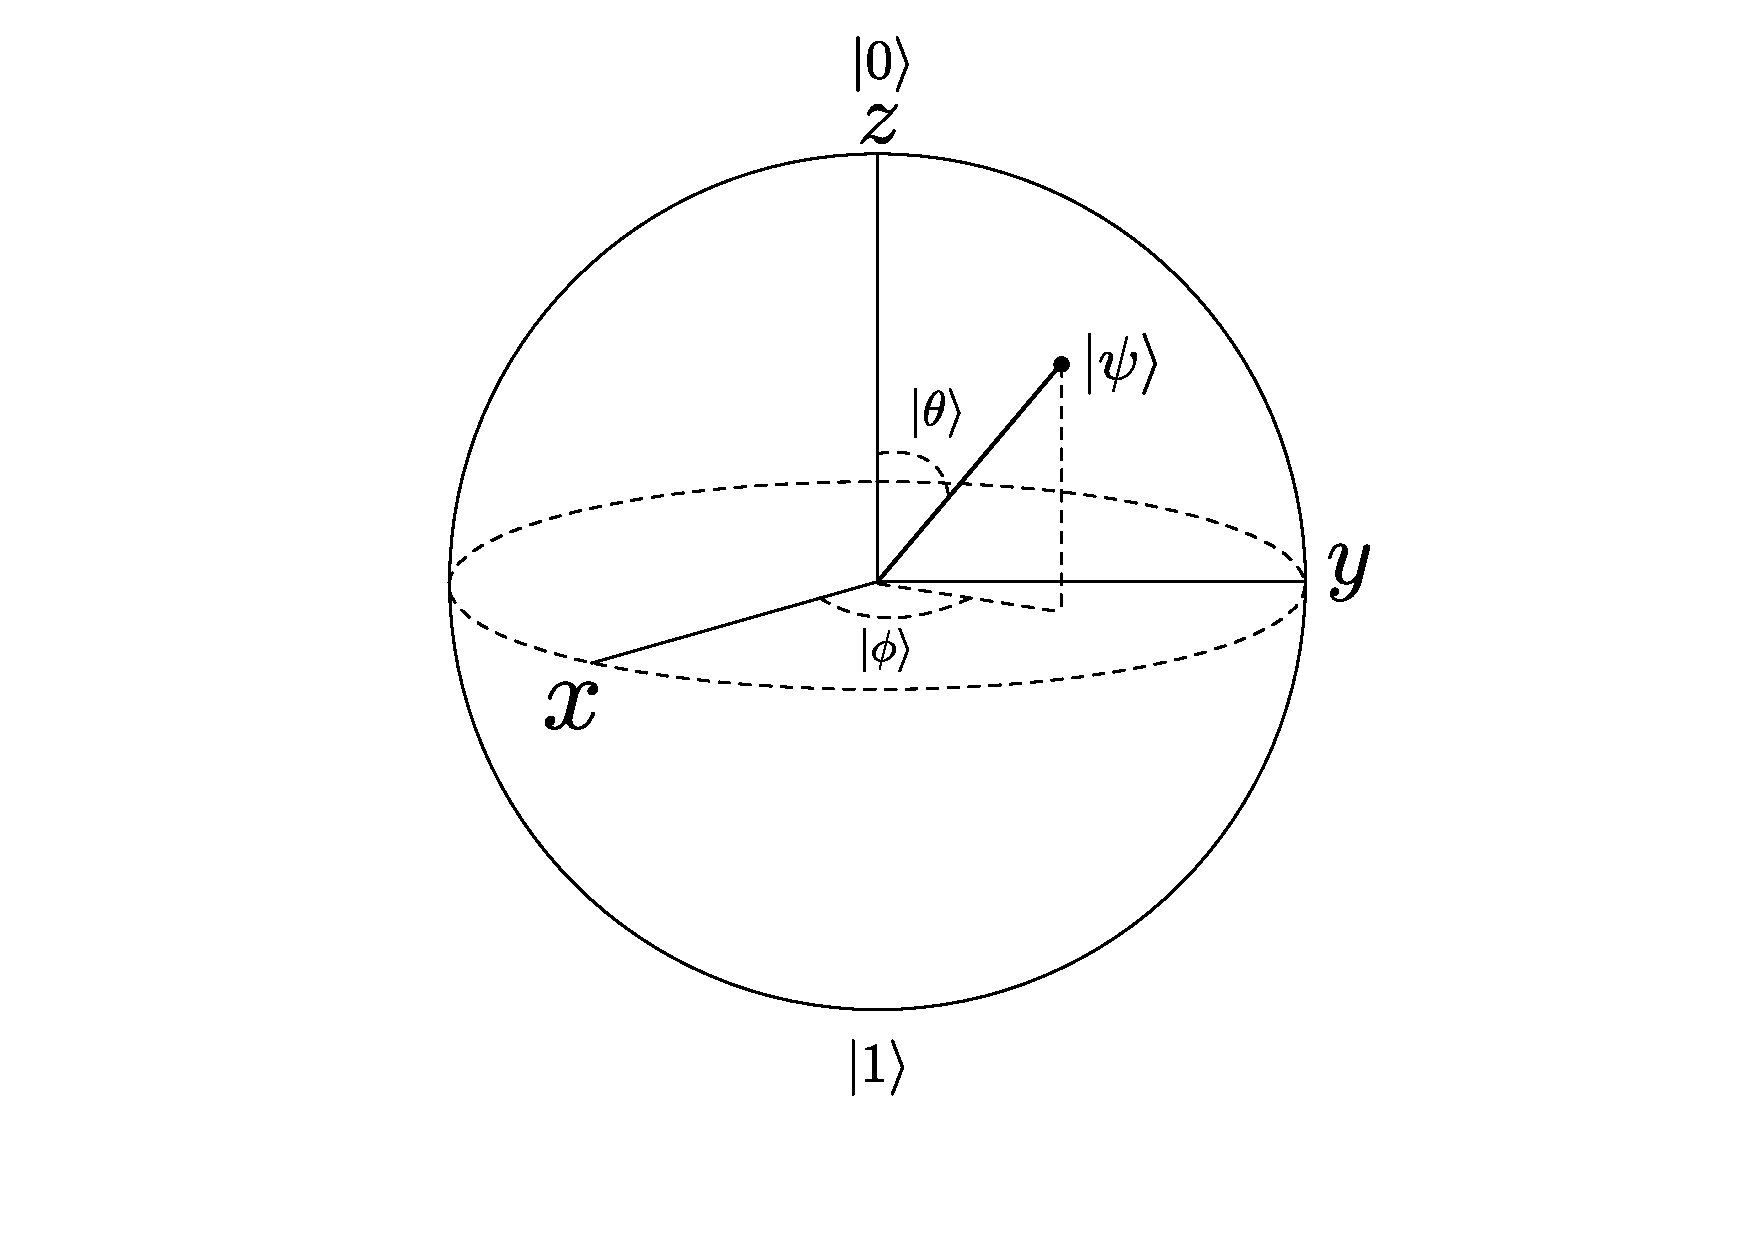
\includegraphics[width = 0.8\columnwidth]{Figures/blochSphere.pdf}
% \caption[Bloch Sphere]{Diagram of the Bloch sphere - the most common representation of a qubit. The poles of the sphere at $\pm z$ represent the $\ket{0}$ and $\ket{1}$ or $\ket{\uparrow}$ and $\ket{\downarrow}$ states. Any point on the surface of the sphere represents some linear superposition of these two states. The state vector of any point is given by: $\ket{\psi} = \cos{\theta/2}\ket{0} + e^{i\phi}\sin{\theta/2}\ket{1}$}
% \label{fig:blochSphere}
% \end{figure}
%
% \section{Donor States in Silicon}
%
% \subsection{The Hyperfine interaction}
%
% Discussion so far has focussed on single electrons in a magnetic field.
% The spins discussed in this thesis will be those of the electrons and nuclei of donors in silicon.
% For these spin states the situation is a little more complicated than the case of a free electron.
% For all the donors discussed here, there is a nuclear as well as electron spin.
% This introduces first an additional term in the Hamiltonian of the system due to the nuclear spin's Zeeman interaction with the magnetic field.
% On top of the separate Zeeman interactions there is an additional interaction between the nucleus and the electron, known as the hyperfine interaction.
% This term is due to the magnetic field of the electron interacting with the magnetic dipole moment of the nucleus.
% This strength of this interaction is proportional to the overlap between the electron and nuclear wavefunctions.
% The result of this is that it is preferential energetically for the electron and nuclear spins to be anti-aligned.
% A further term in the Hamiltonian is due to the nuclear quadrupole but this effect is small enough to be neglected in this treatment.
% These effects leave a Hamiltonian of the following form:
%
% \begin{equation}
% \label{eq:spinHam}
% \hat{H} = \mu_bg_eB_0\hat{S_z} + \mu_ng_nB_0\hat{I_z} + A \hat{S}\cdot\hat{I},
% \end{equation}
%
% where $\mu_b \text{\&} \mu_n$ are the Bohr and nuclear magnetons, $g_e \text{\&} g_n$ are the electron and nuclear g-factors, $\hat{S} \text{\&} \hat{I}$ are the electron and nuclear spin operators, and $A$ is the hyperfine interaction term.
% In general they hyperfine term is a tensor but due to the isotropic nature of silicon can be represented as a scalar here.
%
% \subsection{Spin Transitions}
%
% The electron spin is restricted to be $\pm \frac{1}{2}$, but the nuclear spin can take a much greater range of values.
% The nuclear spin of a phosphorus donor in silicon is $\pm \frac{1}{2}$, by contrast for a bismuth spin it can take the values $-\frac{9}{2}, -\frac{7}{2},...\frac{7}{2},\frac{9}{2}$.
% In the simple case of phosphorus this results in the four energy levels seen in figure \ref{fig:phosLevels}.
%
% \begin{figure}[t!]
% \centering
% \begin{subfigure}[t]{0.7\columnwidth}
% \centering
% 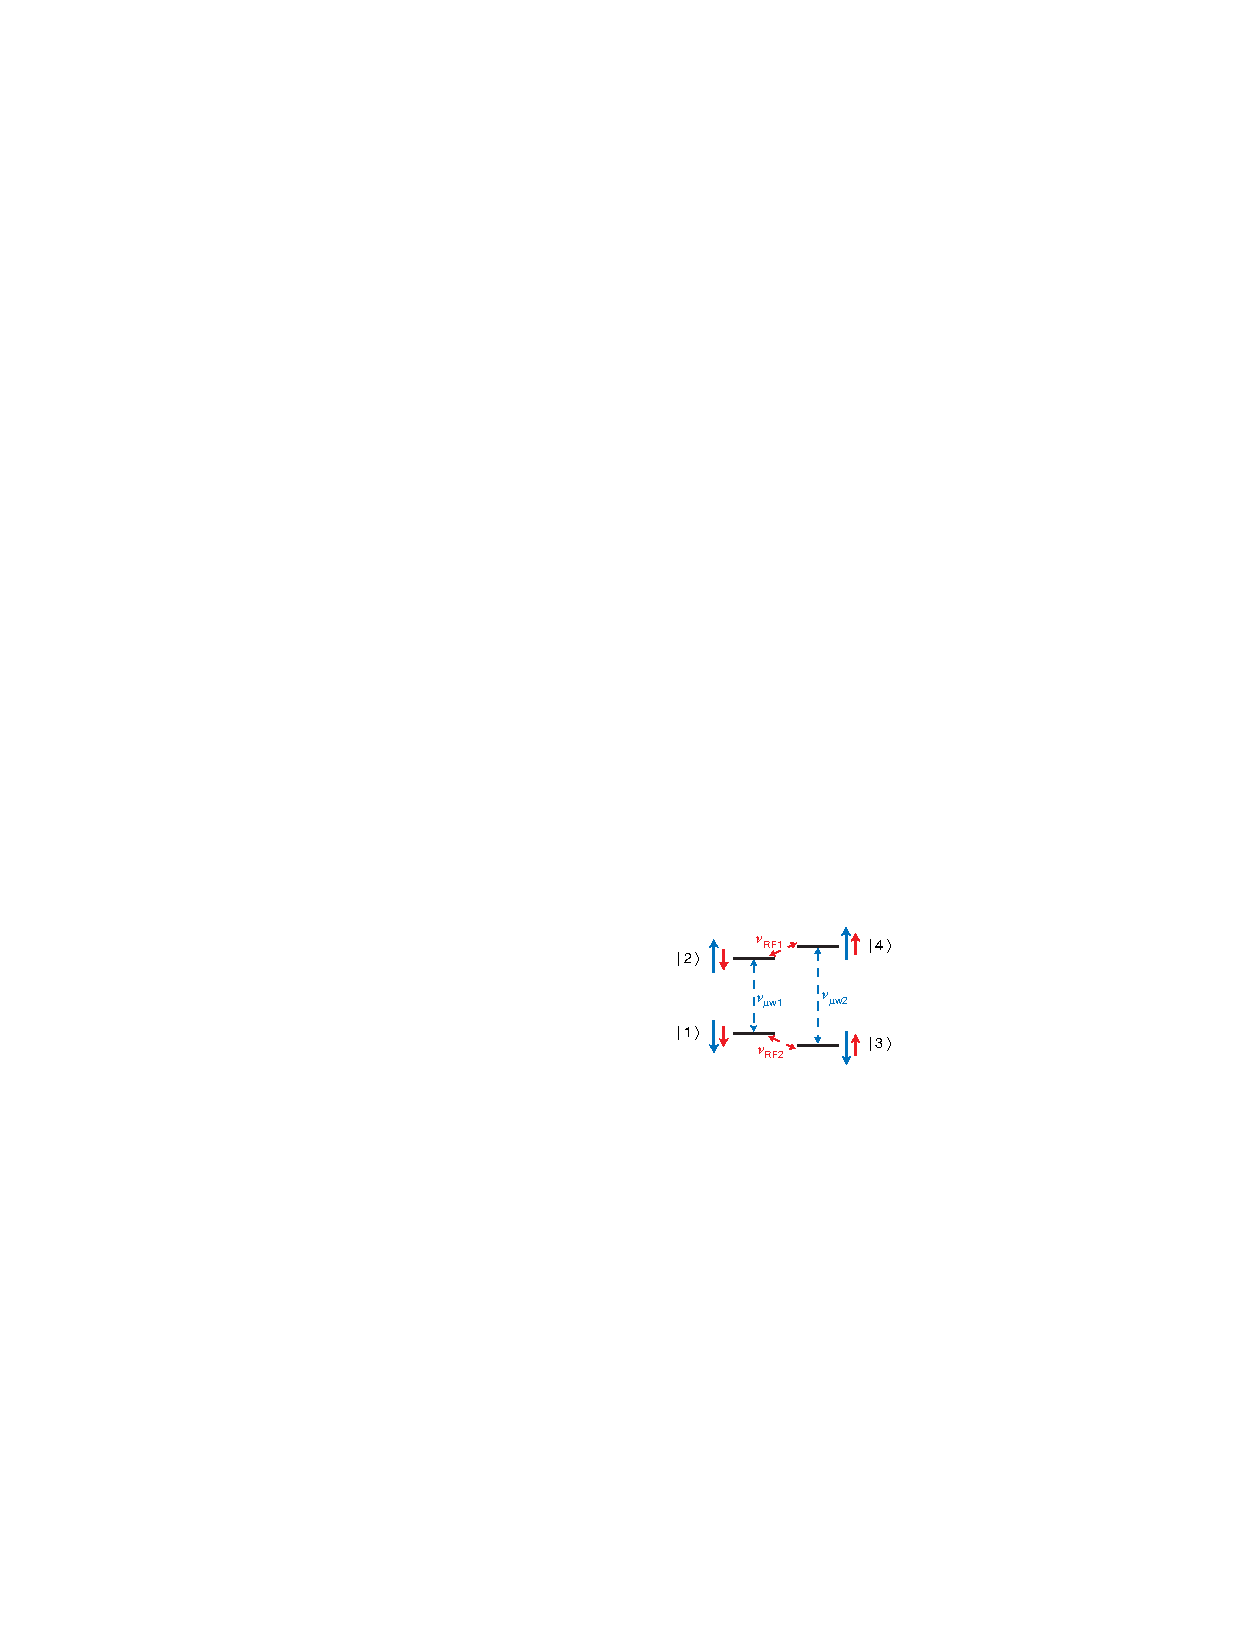
\includegraphics[width = \columnwidth]{Figures/phosphorus.pdf}{(a)}
% \end{subfigure}
% ~
% \begin{subfigure}[t]{0.7\columnwidth}
% \centering
% 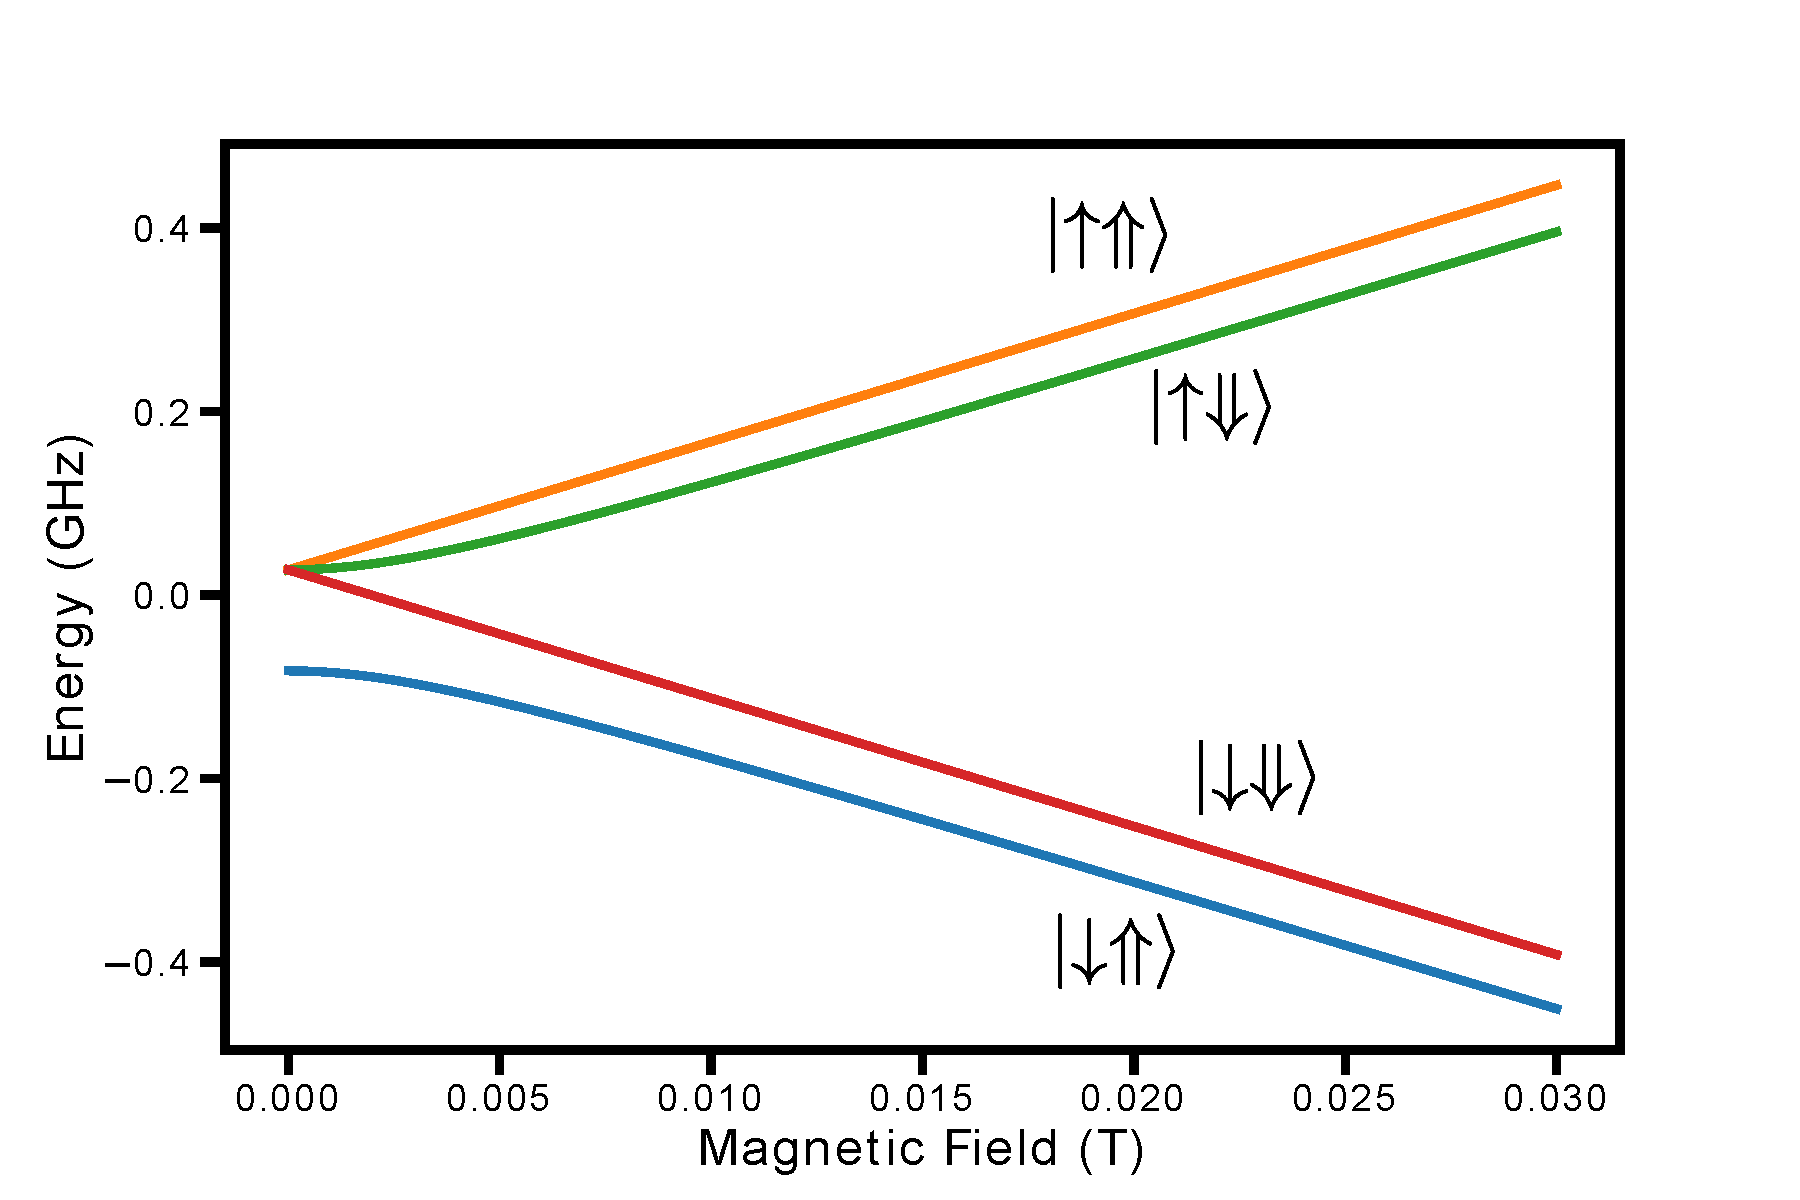
\includegraphics[width = \columnwidth]{Figures/fields.pdf}{(b)}
% \end{subfigure}
% \caption[Phosphorus energy levels and transitions]{Cartoon in a shows the relative energy levels for the different spin states of phosphorus in a high field environment. Note that in this case the electron Zeeman interaction dominates the hyperfine term which dominates the nuclear Zeeman term. b shows the simulated energies for each of the four possible states of the system.}
% \label{fig:phosLevels}
% \end{figure}
%
% For the more complex case of bismuth, instead of 4 possible energy levels there are 20.
% Not all transitions are possible - spins are changed by the absorption or emission of a photon, only allowing transitions where the total spin changes by $\pm1$.
% This means that only nuclear or electron spin can be flipped at once, not both.
% It should be clear that the transitions that involve an electron spin flip ( e.g. $\ket{\uparrow \Uparrow} \longrightarrow \ket{\downarrow \Uparrow}$) are significantly higher in energy than those involving a nuclear spin flip (e.g. $\ket{\uparrow \Uparrow} \longrightarrow \ket{\uparrow \Downarrow}$).
% At typical experimental magnetic fields ($\approx 0.3$ Tesla), the nuclear transitions are at frequencies of 10s of MHz, whilst the electron transitions are at $\approx 9.7$ GHz.
% In addition to their different energies electron and nuclear transitions have different strengths or Rabi frequencies.
% The electron spin transition is much stronger and occurs on the order of nanoseconds at typical pulse powers, with the nuclear transition being on the order of microseconds.
%
% \subsection{Relaxation Processes}
% \label{sec:relProc}
%
% For spins in silicon, three main relaxation or decoherence processes occur, causing the loss of information.
% \\
% \\
% \textbf{Dephasing}
% \\
% \noindent\rule{\columnwidth}{1pt}
% \begin{adjustwidth}{1.5cm}{}
% The first of these was briefly discussed above - dephasing - the time scale for the process is termed \textbf{$T_2^*$}
% This is the process by which an ensemble of spins loses phase coherence due to each spin experiencing a different static magnetic field.
% As was described above, this loss of information can be reversed by a Hahn echo sequence.
% \end{adjustwidth}
% \textbf{Relaxation} \newline
% \noindent\rule{\columnwidth}{1pt}
% \begin{adjustwidth}{1.5cm}{}
% The second process is known as relaxation and its time scale is termed $T_1$. A spin ensemble at a given temperature and magnetic field will have a Boltzmann distributed population across the available spin states defined by the magnetic field axis (i.e. across the eigenstates of the $\hat{Z}$ operator).
% The difference between higher and lower energy states is known as the polarisation of the ensemble.
% If this polarisation is reversed by a $\pi$ pulse, then on a time scale $T_1$ it will relax back to thermal equilibrium.
% As this process almost always involves interaction with the silicon crystal lattice it is also termed \textit{spin-lattice} relaxation.
% This process is strongly correlated with temperature and exact mechanisms will be discussed in the literature review section.
% \end{adjustwidth}
% \textbf{Decoherence}
% \\
% \noindent\rule{\columnwidth}{1pt}
% \begin{adjustwidth}{1.5cm}{}
% The third process, decoherence, occurs on the time scale $T_2$.
% This is similar to the dephasing process described above but is irreversible.
% Irreversible phase differences are caused by by inhomogeneous and \textit{time dependent} magnetic fields.
% Additional phase acquired due to a time varying magnetic field will not be reversed by a Hahn echo sequence as the field will act differently on the spin in the second half of the sequence.
% \end{adjustwidth}
%
% \section{Nitrogen Vacancy Centres in Diamond}
% \subsection{Diamond as a Material}
% \subsection{Energy Level Structure of the Nitrogen Vacancy Centre}
%
%
% \subsection{Summary}
%
% The theory discussed above gives a background to the topics that will be discussed in detail during the literature review section of this report.
